\documentclass[aspectratio=169]{beamer}

% Theme and color scheme
\usetheme{Madrid}
\usecolortheme{default}

% Packages
\usepackage[utf8]{inputenc}
\usepackage{graphicx}
\usepackage{booktabs}
\usepackage{amsmath}
\usepackage{amsfonts}
\usepackage{amssymb}
\usepackage{hyperref}
\usepackage{tikz}
\usepackage{pgfplots}
\pgfplotsset{compat=1.17}

% Title page information
\title{Medical Booking System Dashboard}
\subtitle{Comprehensive BigQuery Healthcare Management and Patient Analytics}
\author{Group 3 - 712}
\institute{Assignment 2}
\date{\today}

% Custom colors
\definecolor{myblue}{RGB}{0,102,204}
\definecolor{mygreen}{RGB}{0,153,76}
\definecolor{myred}{RGB}{204,0,0}
\definecolor{medicalblue}{RGB}{0,123,255}
\definecolor{medicalgreen}{RGB}{40,167,69}

\begin{document}

% Title slide
\begin{frame}
\titlepage
\end{frame}

% Table of contents
\begin{frame}{Outline}
\tableofcontents
\end{frame}

% Section 1: Introduction and Motivation
\section{Introduction and Motivation}

\begin{frame}{Project Overview}
\begin{itemize}
    \item \textbf{Project Goal:} Develop a comprehensive medical booking system using BigQuery and Streamlit for healthcare management
    \item \textbf{Research Question:} How can we create an efficient digital platform for medical appointment scheduling and healthcare analytics?
    \item \textbf{Expected Outcomes:} Streamlined appointment booking, patient management, and healthcare data analytics for improved medical services
\end{itemize}

\vspace{1cm}

\begin{block}{Why This Matters}
Healthcare systems require efficient appointment management and patient data analytics. Our system transforms traditional booking processes into a modern, data-driven platform enabling better patient care, resource optimization, and healthcare insights.
\end{block}
\end{frame}

\begin{frame}{Motivation for Healthcare System Development}
\begin{columns}
\begin{column}{0.6\textwidth}
\textbf{Why We Built This System:}
\begin{itemize}
    \item \textcolor{medicalblue}{Healthcare Efficiency:} Digital transformation of appointment booking processes
    \item \textcolor{medicalgreen}{Patient Experience:} User-friendly interface for seamless medical service access
    \item \textcolor{myred}{Data Analytics:} Comprehensive healthcare data analysis using BigQuery
    \item \textbf{Scalability:} Cloud-based architecture supporting growing healthcare demands
\end{itemize}
\end{column}
\begin{column}{0.4\textwidth}
\begin{center}
\textbf{System Architecture:}\\
BigQuery + Streamlit\\
Healthcare Data Management\\
Real-time Analytics\\
Patient Portal

\vspace{0.5cm}
\textbf{Platform:} Google Cloud\\
\textbf{Frontend:} Streamlit Dashboard\\
\textbf{Backend:} BigQuery Database
\end{center}
\end{column}
\end{columns}
\end{frame}

% Section 2: System Overview
\section{System Overview}

\begin{frame}{System Description}
\begin{table}[h]
\centering
\begin{tabular}{@{}ll@{}}
\toprule
\textbf{Component} & \textbf{Details} \\
\midrule
Application Type & Medical Booking \& Management System \\
Platform & Google BigQuery + Streamlit \\
Authentication & User-based with Admin privileges \\
Data Storage & BigQuery Cloud Database \\
User Interface & Interactive Web Dashboard \\
\bottomrule
\end{tabular}
\end{table}

\vspace{0.5cm}

\begin{alertblock}{Key System Characteristics}
Comprehensive healthcare management platform with patient booking, specialist management, appointment tracking, and administrative analytics. Features role-based access control and real-time data visualization.
\end{alertblock}
\end{frame}

\begin{frame}{System Features Overview}
\begin{columns}
\begin{column}{0.5\textwidth}
\textbf{Core Features:}
\begin{itemize}
    \item \textbf{User Authentication:} Secure login/signup system
    \item \textbf{Appointment Booking:} Interactive scheduling interface
    \item \textbf{Specialist Management:} Doctor profiles and specialties
    \item \textbf{Patient Dashboard:} Personal appointment tracking
\end{itemize}
\end{column}
\begin{column}{0.5\textwidth}
\textbf{Advanced Features:}
\begin{itemize}
    \item \textbf{Admin Dashboard:} Comprehensive analytics and management
    \item \textbf{BigQuery Integration:} Real-time healthcare data analysis
    \item \textbf{Data Visualization:} Interactive charts and reports
    \item \textbf{Performance Analytics:} System health monitoring
\end{itemize}
\end{column}
\end{columns}

\vspace{1cm}

\begin{block}{Healthcare Focus}
\textbf{Medical Objectives:} Patient care optimization, appointment efficiency, specialist utilization analysis, and healthcare data insights for improved medical service delivery.
\end{block}
\end{frame}

% Section 3: Technical Architecture
\section{Technical Architecture}

\begin{frame}{System Architecture}
\begin{enumerate}
    \item \textbf{Data Infrastructure}
    \begin{itemize}
        \item BigQuery cloud database for healthcare data storage
        \item Faker-generated synthetic healthcare datasets
        \item Service account authentication for secure access
        \item Real-time data synchronization and updates
    \end{itemize}
    
    \item \textbf{Application Development}
    \begin{itemize}
        \item Streamlit web framework for interactive dashboard
        \item Modular architecture with separate components
        \item User session management and authentication
    \end{itemize}
    
    \item \textbf{Healthcare Analytics}
    \begin{itemize}
        \item Patient appointment tracking and analysis
        \item Specialist performance monitoring
        \item Healthcare system health indicators
    \end{itemize}
\end{enumerate}
\end{frame}

\begin{frame}{Technology Stack}
\begin{center}
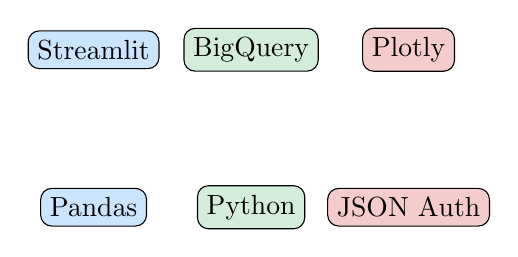
\begin{tikzpicture}[node distance=2cm]
% Create nodes for different tools
\node[draw, rounded corners, fill=medicalblue!20] (streamlit) {Streamlit};
\node[draw, rounded corners, fill=medicalgreen!20, right of=streamlit] (bigquery) {BigQuery};
\node[draw, rounded corners, fill=myred!20, right of=bigquery] (plotly) {Plotly};
\node[draw, rounded corners, fill=medicalblue!20, below of=streamlit] (pandas) {Pandas};
\node[draw, rounded corners, fill=medicalgreen!20, below of=bigquery] (python) {Python};
\node[draw, rounded corners, fill=myred!20, below of=plotly] (json) {JSON Auth};

% Add connections if desired
\end{tikzpicture}
\end{center}

\vspace{0.5cm}

\textbf{Technology Stack:}
\begin{itemize}
    \item \textbf{Frontend:} Streamlit web framework with option-menu navigation
    \item \textbf{Database:} Google BigQuery for healthcare data storage
    \item \textbf{Data Generation:} Faker library for synthetic healthcare data creation
    \item \textbf{Visualizations:} Plotly Express, Plotly Graph Objects for analytics
    \item \textbf{Data Processing:} Pandas, NumPy for healthcare data manipulation
    \item \textbf{Authentication:} JSON-based user management system
\end{itemize}
\end{frame}

% Section 4: System Features
\section{System Features}

\begin{frame}{Dashboard Features and Capabilities}
\begin{columns}
\begin{column}{0.5\textwidth}
\textbf{User Interface Features:}
\begin{itemize}
    \item \textcolor{medicalblue}{Role-based Navigation}
    \item \textcolor{medicalgreen}{Interactive Appointment Booking}
    \item \textcolor{myred}{Real-time Data Updates}
    \item \textbf{Responsive Design}
\end{itemize}

\vspace{0.5cm}

\textbf{Healthcare Capabilities:}
\begin{itemize}
    \item Specialist profile management
    \item Appointment scheduling and tracking
    \item Patient data analytics
    \item Healthcare system monitoring
\end{itemize}
\end{column}
\begin{column}{0.5\textwidth}
\textbf{System Pages:}
\begin{itemize}
    \item \textbf{Home:} Dashboard overview and KPIs
    \item \textbf{Login/Signup:} User authentication
    \item \textbf{Specialists:} Doctor profiles and specialties
    \item \textbf{Book Appointment:} Interactive scheduling
    \item \textbf{My Appointments:} Patient appointment tracking
    \item \textbf{Admin Dashboard:} System management and analytics
\end{itemize}

\vspace{0.5cm}
\begin{alertblock}{Key Innovation}
Seamless integration of healthcare data management with user-friendly appointment booking system
\end{alertblock}
\end{column}
\end{columns}
\end{frame}

\begin{frame}{Healthcare Analytics and Insights}
\begin{block}{Key System Capabilities}
\begin{itemize}
    \item \textbf{Patient Management:} Comprehensive appointment tracking and user analytics
    \item \textbf{Specialist Analytics:} Performance monitoring and specialty distribution analysis
    \item \textbf{System Health:} Real-time monitoring of booking patterns and system performance
\end{itemize}
\end{block}

\vspace{0.5cm}

\begin{columns}
\begin{column}{0.5\textwidth}
\textbf{Analytics Features:}
\begin{itemize}
    \item Real-time appointment statistics
    \item Specialist utilization tracking
    \item Patient engagement metrics
    \item System performance monitoring
\end{itemize}
\end{column}
\begin{column}{0.5\textwidth}
\textbf{Visualization Types:}
\begin{itemize}
    \item Appointment trends (Line Charts)
    \item Specialist distribution (Pie Charts)
    \item Patient demographics (Bar Charts)
    \item System health indicators (Metrics)
    \item Booking patterns (Time Series)
    \item Performance analytics (Dashboard)
\end{itemize}
\end{column}
\end{columns}
\end{frame}

% Section 5: Data Management
\section{Data Management}

\begin{frame}{BigQuery Healthcare Data Integration}
\begin{block}{Healthcare Data Tables}
\begin{itemize}
    \item \textbf{Medical Specialists:} Doctor profiles, specialties, ratings, and contact information
    \item \textbf{Appointments:} Patient bookings, scheduling data, and status tracking
    \item \textbf{Patients:} User demographics and healthcare information
    \item \textbf{Time Slots:} Available appointment times and scheduling constraints
    \item \textbf{Dates:} Calendar management and availability tracking
\end{itemize}
\end{block}

\vspace{0.3cm}

\begin{alertblock}{Data Generation}
All healthcare data was generated using \textbf{Faker}, a Python library for creating realistic synthetic data. This approach ensures data privacy while providing comprehensive test datasets for system development and demonstration.
\end{alertblock}

\vspace{0.5cm}

\begin{columns}
\begin{column}{0.5\textwidth}
\textbf{Data Analytics:}
\begin{itemize}
    \item Real-time appointment tracking
    \item Specialist performance metrics
    \item Patient engagement analysis
    \item System utilization statistics
\end{itemize}
\end{column}
\begin{column}{0.5\textwidth}
\textbf{Data Quality:}
\begin{itemize}
    \item Automated data validation
    \item Real-time synchronization
    \item Error handling and recovery
    \item Data integrity monitoring
\end{itemize}
\end{column}
\end{columns}
\end{frame}

\begin{frame}{User Authentication and Security}
\begin{block}{Security Features}
\begin{itemize}
    \item \textbf{User Authentication:} Secure login/signup with password hashing
    \item \textbf{Role-based Access:} Patient and Admin user privileges
    \item \textbf{Session Management:} Secure user session handling
    \item \textbf{Data Protection:} Encrypted data transmission and storage
\end{itemize}
\end{block}

\vspace{0.5cm}

\begin{columns}
\begin{column}{0.5\textwidth}
\textbf{User Types:}
\begin{itemize}
    \item \textbf{Patients:} Book appointments, view personal data
    \item \textbf{Administrators:} Full system access, analytics, management
    \item \textbf{Guests:} Limited access to login/signup only
\end{itemize}
\end{column}
\begin{column}{0.5\textwidth}
\textbf{Security Measures:}
\begin{itemize}
    \item Password hashing (SHA-256)
    \item Session state management
    \item Protected route access
    \item Input validation and sanitization
\end{itemize}
\end{column}
\end{columns}
\end{frame}

% Section 6: Conclusions
\section{Conclusions and Future Work}

\begin{frame}{Key Achievements}
\begin{enumerate}
    \item \textbf{Technical Implementation:}
    \begin{itemize}
        \item Successfully integrated BigQuery with Streamlit for healthcare data management
        \item Developed comprehensive medical booking system with 6 main functional modules
        \item Implemented robust authentication system and role-based access control
    \end{itemize}
    
    \item \textbf{Healthcare System Success:}
    \begin{itemize}
        \item Created efficient appointment booking and management system
        \item Developed comprehensive admin dashboard for healthcare analytics
        \item Implemented real-time data visualization and system monitoring
    \end{itemize}
    
    \item \textbf{Practical Impact:}
    \begin{itemize}
        \item System enables streamlined healthcare appointment management
        \item Interactive interface improves patient experience and accessibility
        \item Scalable architecture supports growing healthcare facility needs
    \end{itemize}
\end{enumerate}
\end{frame}

\begin{frame}{Future Enhancements}
\begin{block}{Potential Improvements}
\begin{itemize}
    \item \textbf{Advanced Features:} SMS/Email notifications, calendar integration, payment processing
    \item \textbf{Analytics Enhancement:} Machine learning for appointment prediction, patient behavior analysis
    \item \textbf{Mobile Application:} Native mobile app for improved accessibility
    \item \textbf{Integration:} Electronic Health Records (EHR) system integration
\end{itemize}
\end{block}

\vspace{0.5cm}

\begin{columns}
\begin{column}{0.5\textwidth}
\textbf{Technical Roadmap:}
\begin{itemize}
    \item API development for third-party integrations
    \item Advanced reporting and analytics
    \item Multi-language support
    \item Enhanced security features
\end{itemize}
\end{column}
\begin{column}{0.5\textwidth}
\textbf{Healthcare Features:}
\begin{itemize}
    \item Telemedicine integration
    \item Prescription management
    \item Medical history tracking
    \item Insurance verification
\end{itemize}
\end{column}
\end{columns}
\end{frame}

% Section 7: Questions and Discussion
\section{Questions and Discussion}

\begin{frame}{Questions and Discussion}
\begin{center}
\Huge Thank You!

\vspace{1cm}

\Large Questions and Discussion

\vspace{1cm}

\normalsize
\textbf{Group 712 Team Members:}\\
Nyiko Maluleke (3928378) | Mlamli Mkize (3948221)\\
Bulelani Kote (4523387) | Alizwa Mdaka (3666983)\\
Siyabonga Masango (3857285)

\vspace{0.5cm}
\textbf{Project:} Medical Booking System Dashboard\\
\textbf{Technology:} BigQuery + Streamlit + Python\\
\textbf{Focus:} Healthcare Management \& Patient Analytics
\end{center}
\end{frame}

% Appendix
\appendix
\section{Appendix}

\begin{frame}{Technical Implementation Details}
\begin{itemize}
    \item \textbf{System Architecture:} Modular Streamlit application with BigQuery backend
    \item \textbf{Data Source:} Google BigQuery healthcare tables (specialists, appointments, patients, timeslots)
    \item \textbf{Data Generation:} Faker library for creating realistic synthetic healthcare data
    \item \textbf{Authentication:} JSON-based user management with SHA-256 password hashing
    \item \textbf{Deployment:} Streamlit Cloud with GitHub integration
\end{itemize}

\vspace{1cm}

\begin{block}{Key Features Implemented}
\begin{itemize}
    \item 6 main application modules (Home, Login, Specialists, Booking, Appointments, Admin)
    \item Real-time BigQuery data integration and analytics
    \item Interactive appointment booking with specialist selection
    \item Comprehensive admin dashboard with healthcare analytics
    \item Role-based access control (Patient/Admin)
    \item Responsive design with modern UI/UX
\end{itemize}
\end{block}
\end{frame}

\begin{frame}{System Modules Overview}
\begin{block}{Application Structure}
\begin{itemize}
    \item \textbf{streamlit\_app.py:} Main application with navigation and routing
    \item \textbf{modules/home.py:} Dashboard with KPIs and system analytics
    \item \textbf{modules/login.py:} User authentication and registration
    \item \textbf{modules/specialists.py:} Doctor profiles and specialty management
    \item \textbf{modules/book\_appointment.py:} Interactive appointment scheduling
    \item \textbf{modules/my\_appointments.py:} Patient appointment tracking
    \item \textbf{modules/admin\_dashboard.py:} Administrative analytics and management
    \item \textbf{modules/utilis.py:} Utility functions and BigQuery integration
\end{itemize}
\end{block}
\end{frame}

% Acknowledgement slide
\begin{frame}{Acknowledgement}
\begin{block}{Development Support}
This healthcare management system was developed with the assistance of \textbf{Cursor}, an AI-powered coding assistant, which supported the development, structuring, and debugging of the Python code and system architecture.
\end{block}
\end{frame}

\end{document}
